\section{Aim}

A large number of targets are those that are not being tracked for the visibility and hence these targets are updated using the rules defined by the team. These are simple rule such as what percentage of the bid should be increased/decreased if the match type/target type and the last bid of the target is known.

\section{Assumptions}

\begin{enumerate}
    \item The performance of a target depend on the bid. Higher the bid, higher the sales.
    \item The bid change reflects in the performance of the target very quickly.
\end{enumerate}

\section{The Rules}

The rules are mainly divided into three parts:

\begin{enumerate}
    \item \textbf{Increase Gradually}
    \item \textbf{Decrease Gradually}
    \item \textbf{No Changes}
\end{enumerate}

The bids are increased or decreased based on these three actions. We use the average CPC of the whole category for this.

\subsection{Average CPC}

\subsection*{calculate\_avg\_cpc Function}

\begin{lstlisting}[language=Python]
def calculate_avg_cpc(client_profile_id):
    # ... (code omitted for brevity)
    return cpc
\end{lstlisting}

This function calculates the average cost per click (CPC) for a given client profile id for the last 7 days. The function takes as input a string `client\_profile\_id` which is the client profile id of the client.

The function first constructs a SQL query to calculate the average CPC from the `AMS\_Automation\_Consolidated.dbo.table\_targeting` table where the `client\_profile\_id` matches the input and the date is between the current date minus 8 and the current date minus 1.

The function then runs the query and retrieves the average CPC. If the average CPC is null or zero, the function raises an `UnexpectedResultFound` error. If the average CPC is not null or zero, the function logs the CPC and returns it.

\begin{figure}[ht]
    \centering
    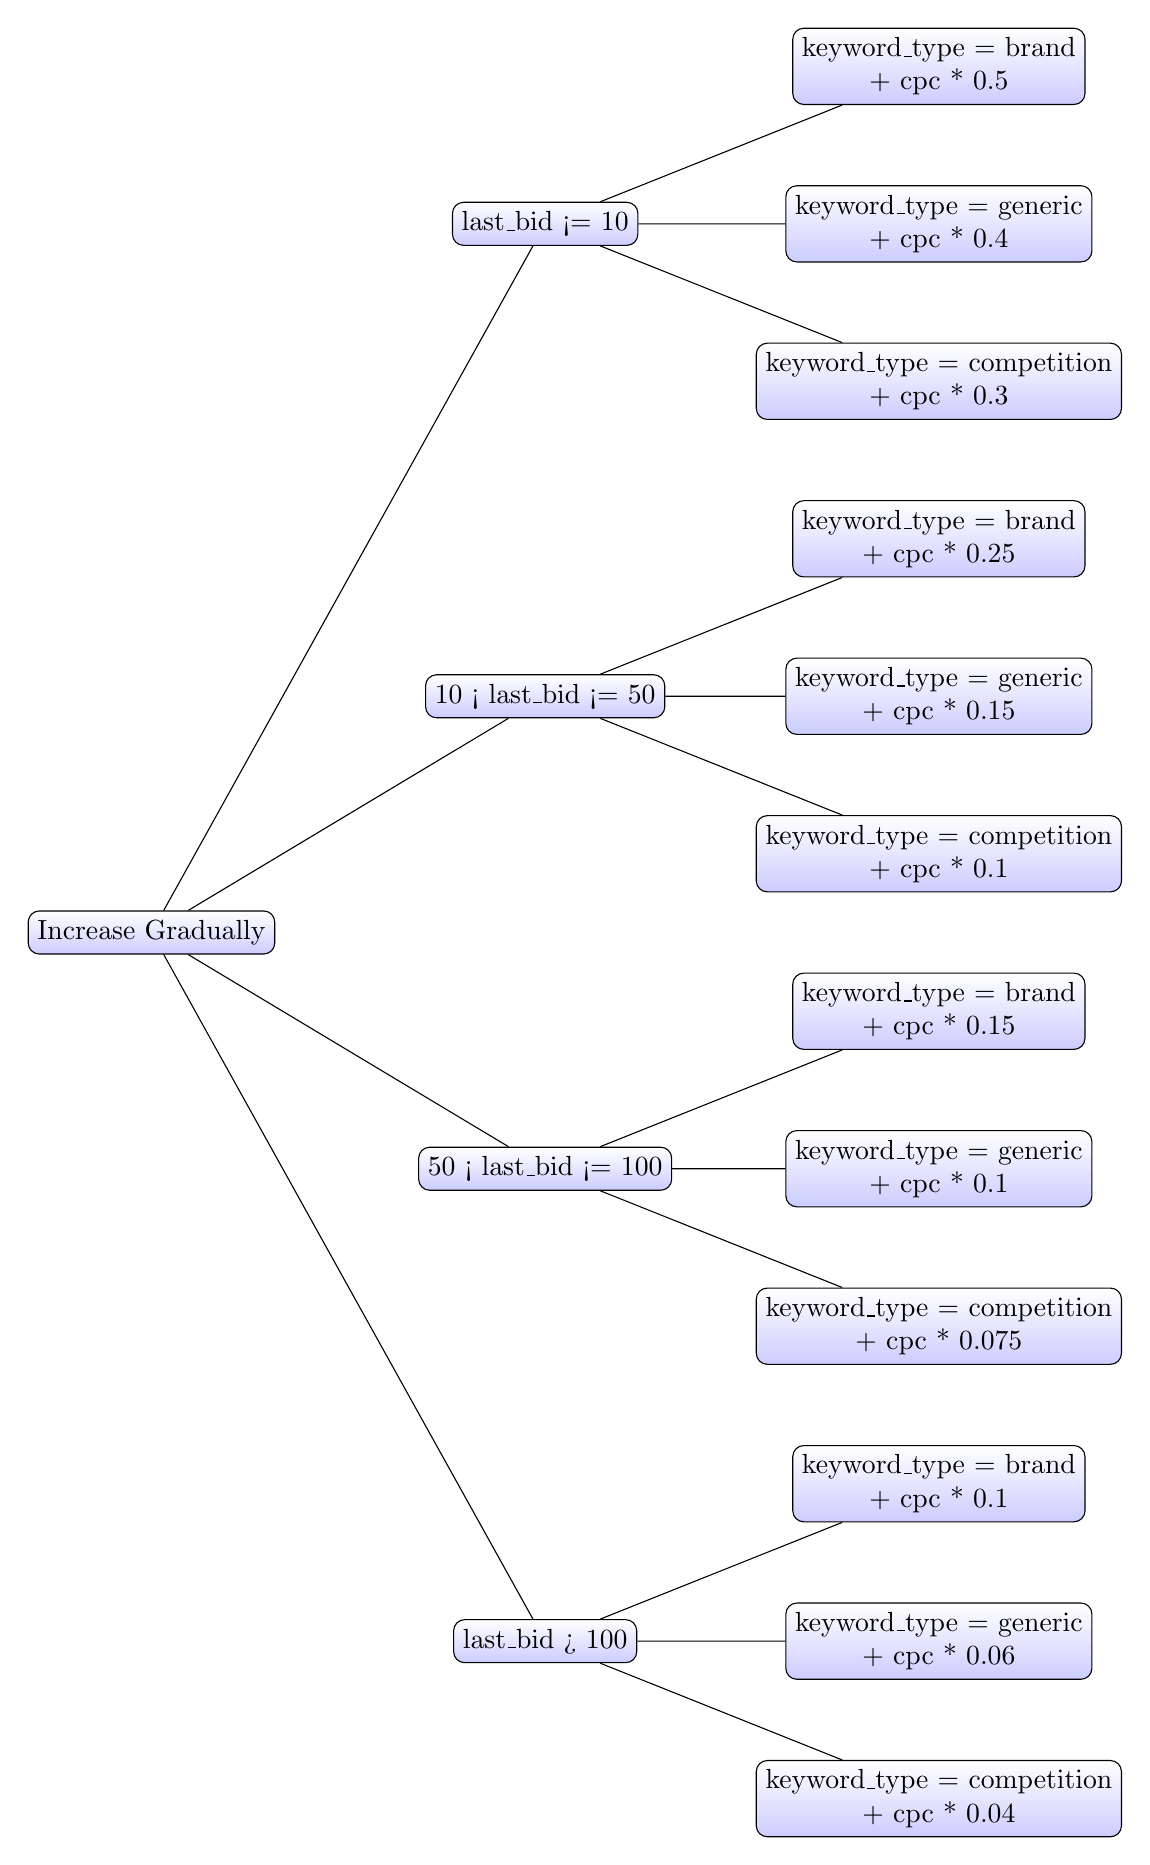
\begin{tikzpicture}[
            grow'=right,
            level 1/.style={level distance=5cm, sibling distance=6cm},
            level 2/.style={level distance=5cm, sibling distance=2cm},
            every node/.style = {shape=rectangle, rounded corners, draw, align=center, top color=white, bottom color=blue!20}
        ]
        \node {Increase Gradually}
        child { node {last\_bid <= 10}
                child { node {keyword\_type = brand \\ + cpc * 0.5} }
                child { node {keyword\_type = generic \\ + cpc * 0.4} }
                child { node {keyword\_type = competition \\ + cpc * 0.3} }
            }
        child { node {10 < last\_bid <= 50}
                child { node {keyword\_type = brand \\ + cpc * 0.25} }
                child { node {keyword\_type = generic \\ + cpc * 0.15} }
                child { node {keyword\_type = competition \\ + cpc * 0.1} }
            }
        child { node {50 < last\_bid <= 100}
                child { node {keyword\_type = brand \\ + cpc * 0.15} }
                child { node {keyword\_type = generic \\ + cpc * 0.1} }
                child { node {keyword\_type = competition \\ + cpc * 0.075} }
            }
        child { node {last\_bid > 100}
                child { node {keyword\_type = brand \\ + cpc * 0.1} }
                child { node {keyword\_type = generic \\ + cpc * 0.06} }
                child { node {keyword\_type = competition \\ + cpc * 0.04} }
            };
    \end{tikzpicture}
    \caption{Percentage increase in bid}
    \label{fig:increase_gradually_rule}
\end{figure}


\subsection{Increase Gradually}

The bids are increased gradually based on the last bid of the target. Here is a figure that shows the percentage increase in the bid based on the last bid of the target. See the figure \ref{fig:increase_gradually_rule}.

\subsection{Decrease Gradually}

The below figure shows the percentage decrease in the bid based on the last bid of the target. See the figure \ref{fig:decrease_gradually_rule}.

\begin{figure}[ht]
    \centering
    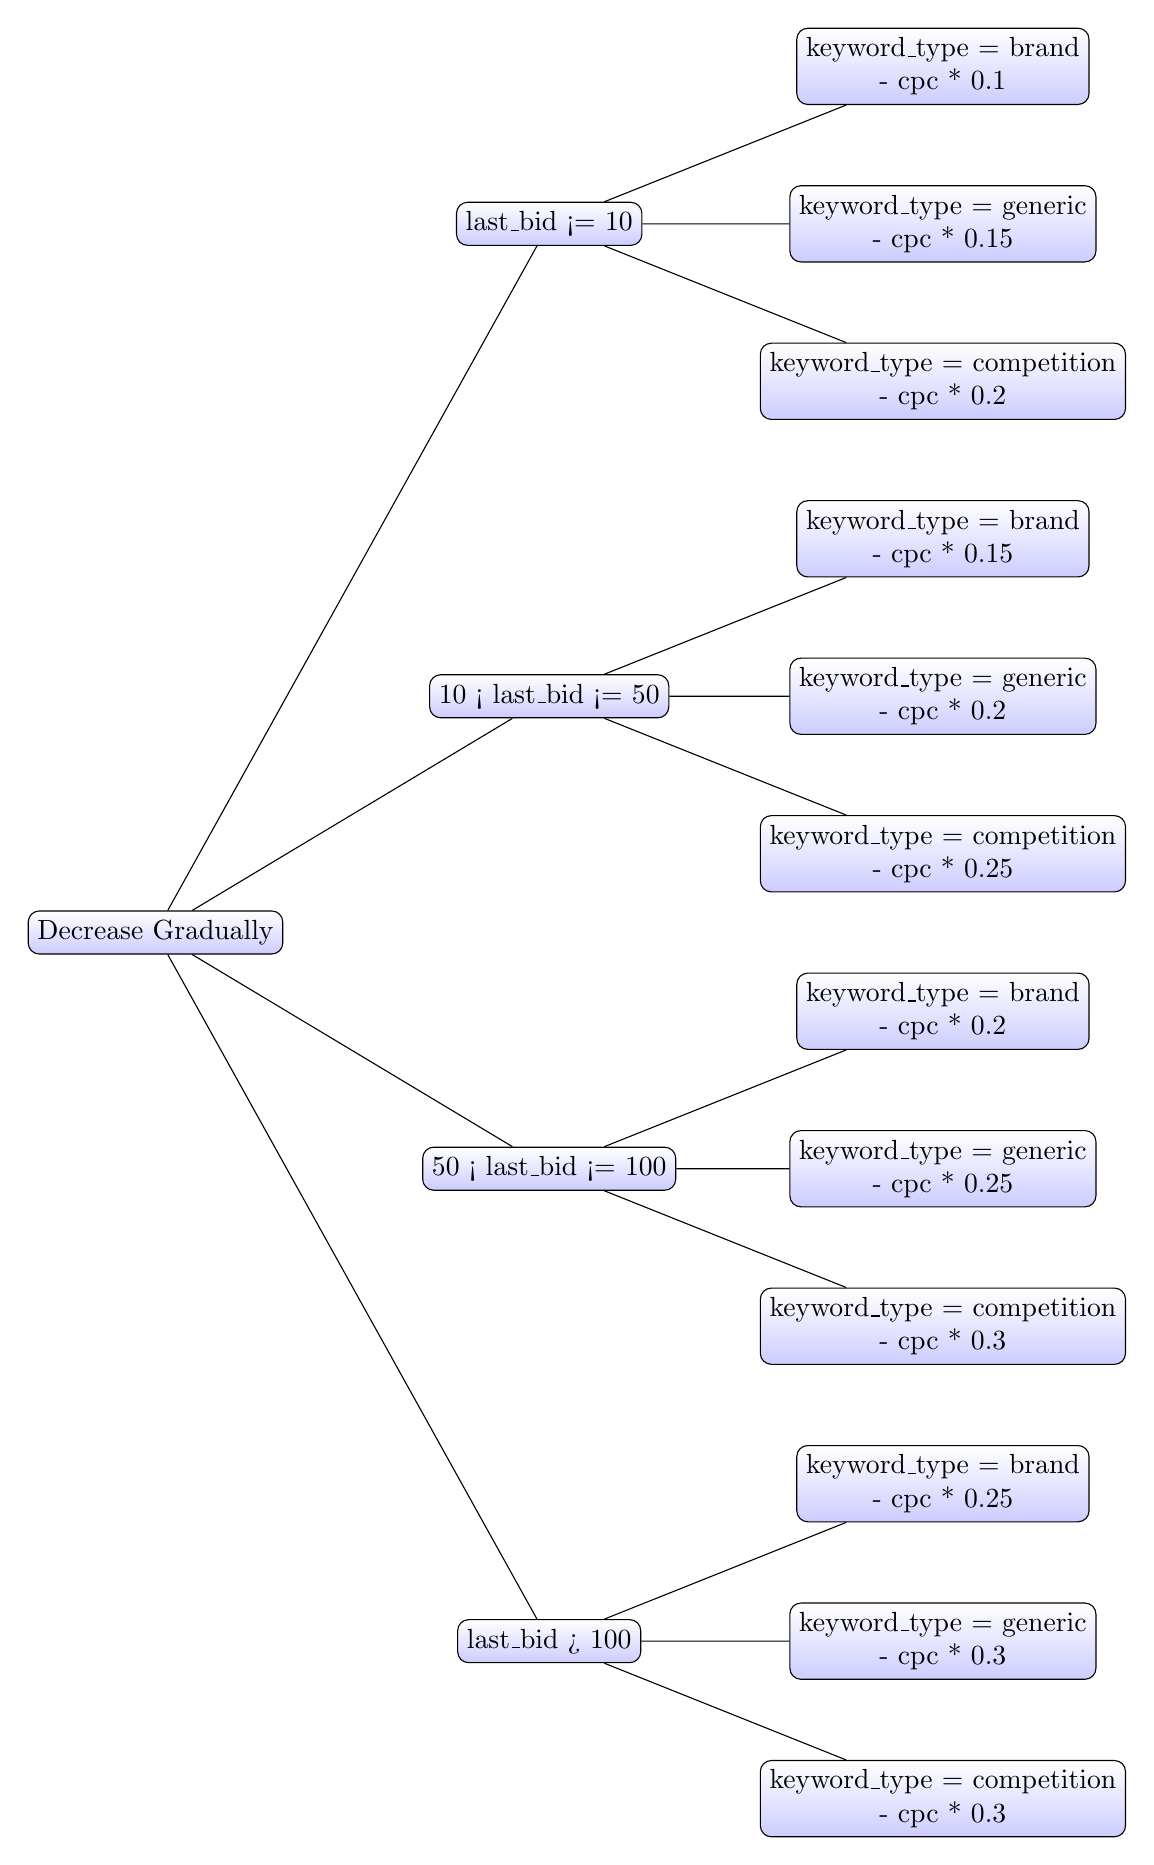
\begin{tikzpicture}[
            grow'=right,
            level 1/.style={level distance=5cm, sibling distance=6cm},
            level 2/.style={level distance=5cm, sibling distance=2cm},
            every node/.style = {shape=rectangle, rounded corners, draw, align=center, top color=white, bottom color=blue!20}
        ]

        \node {Decrease Gradually}
        child { node {last\_bid <= 10}
                child { node {keyword\_type = brand \\ - cpc * 0.1} }
                child { node {keyword\_type = generic \\ - cpc * 0.15} }
                child { node {keyword\_type = competition \\ - cpc * 0.2} }
            }
        child { node {10 < last\_bid <= 50}
                child { node {keyword\_type = brand \\ - cpc * 0.15} }
                child { node {keyword\_type = generic \\ - cpc * 0.2} }
                child { node {keyword\_type = competition \\ - cpc * 0.25} }
            }
        child { node {50 < last\_bid <= 100}
                child { node {keyword\_type = brand \\ - cpc * 0.2} }
                child { node {keyword\_type = generic \\ - cpc * 0.25} }
                child { node {keyword\_type = competition \\ - cpc * 0.3} }
            }
        child { node {last\_bid > 100}
                child { node {keyword\_type = brand \\ - cpc * 0.25} }
                child { node {keyword\_type = generic \\ - cpc * 0.3} }
                child { node {keyword\_type = competition \\ - cpc * 0.3} }
            };
    \end{tikzpicture}
    \caption{Percentage decrease in bid}
    \label{fig:decrease_gradually_rule}
\end{figure}